% !TEX root =../ECE343_Slides_Rogers.tex

\begin{frame}{}
\renewcommand{\arraystretch}{1}
	\begin{textblock}{14}(0.5,1.75)
	\def\myfontsize{footnotesize}
	\setcounter{mylnum}{24}
%\def\myfontsize{normalsize}
\begin{center}
\begin{\myfontsize}
\begin{tabular}{| c | l | c | l |}
\hline
\textbf{Lesson} 		  	& \textbf{Topics}             & \pbox{5cm}{\textbf{Reading}}	& \textbf{Notes}		\\ \hline\hline
\ifnum\lessonNum=\value{mylnum} \rowcolor{green!20!white}\fi
	\themylnum  
	& BVP (Capacitor, Coax), Electric Potential	
	& 5.16
	&  LO 5.3  
\stepcounter{mylnum}\\ \hline \hline
\ifnum\lessonNum=\value{mylnum} \rowcolor{green!20!white}\fi
	\themylnum 	
	& Electric Boundary Conditions
	& 5.18-5.22	
	& LO 5.4			
\stepcounter{mylnum}\\ \hline
\ifnum\lessonNum=\value{mylnum} \rowcolor{green!20!white}\fi
	\themylnum 	
	& BC's/Capacitance			
	& 5.23-5.24
	& 	
\stepcounter{mylnum}\\ \hline
\ifnum\lessonNum=\value{mylnum} \rowcolor{green!20!white}\fi
	\themylnum 	
	& Electrostatic Lab			
	& Lab packet
	& 	
\stepcounter{mylnum}\\ \hline
\rowcolor{gray!20!white}\multicolumn{4}{| c |}{\textbf{Chapter 6: Steady Current \& Conductivity}}	\\ \hline\hline
\ifnum\lessonNum=\value{mylnum} \rowcolor{green!20!white}\fi
	\themylnum 	
	& Current density, Conductivity, Resistance
	& Ch. 6
	&   					
\stepcounter{mylnum}\\ \hline\hline
\rowcolor{gray!20!white}\multicolumn{4}{| c |}{\textbf{Chapter 7: Magnetostatics}}						\\ \hline\hline
\ifnum\lessonNum=\value{mylnum} \rowcolor{green!20!white}\fi
	\themylnum 	
	&  Magnetic Fields, Gauss' Law for Magnetism	
	& 7.1-7.3		
	&LO 7.1-7.2 \textbf{GR 2} 				
\stepcounter{mylnum}\\ \hline
\ifnum\lessonNum=\value{mylnum} \rowcolor{green!20!white}\fi
	\themylnum 	
	& Ampere's Law 	
	& 7.4-7.5, 7.9
	& LO 7.3		
\stepcounter{mylnum}\\ \hline 
\ifnum\lessonNum=\value{mylnum} \rowcolor{green!20!white}\fi
	\themylnum 	
	&  Ampere's Law Applied
	&  7.6-7.8
	& LO 7.3
\stepcounter{mylnum}\\ \hline 
\ifnum\lessonNum=\value{mylnum} \rowcolor{green!20!white}\fi
	\themylnum	
	& Magnetic Boundary Conditions	
	& 7.10-7.14	
	& LO 7.4 		
\stepcounter{mylnum}\\ \hline 
\ifnum\lessonNum=\value{mylnum} \rowcolor{green!20!white}\fi
	\themylnum  
	& Magnetostatics Lab
	& Lab packet
	&  		
\stepcounter{mylnum}\\ \hline \hline
\rowcolor{gray!20!white}\multicolumn{4}{| c |}{\textbf{Chapter 8: Time-Varying Fields}}					\\ \hline\hline
\ifnum\lessonNum=\value{mylnum} \rowcolor{green!20!white}\fi
	\themylnum 	
	& Faraday's Law, Displacement Current, Maxwell Eqns
	& 8.3, 8.8, 8.9
	& LO 8.1
\stepcounter{mylnum}\\ \hline 
\ifnum\lessonNum=\value{mylnum} \rowcolor{green!20!white}\fi
	\themylnum	
	& Faraday's Law, Displacement Current, Maxwell Eqns 
	&  8.3, 8.8, 8.9
	& LO 8.2-8.3
\stepcounter{mylnum}\\ \hline 

\rowcolor{gray!20!white}\multicolumn{4}{| c |}{\textbf{Chapter 9: Plane Waves in Lossless Media}}					\\ \hline\hline
\ifnum\lessonNum=\value{mylnum} \rowcolor{green!20!white}\fi
	\themylnum	
	& Maxwell's Equations in lossless, source-free region		
	& 9.1-9.2
	& LO 9.1	 
\stepcounter{mylnum}\\ \hline
\ifnum\lessonNum=\value{mylnum} \rowcolor{green!20!white}\fi
	\themylnum	
	& Maxwell's Equations in lossless, source-free region		
	& 9.1-9.2
	& LO 9.1	 
\stepcounter{mylnum}\\ \hline
%\ifnum\lessonNum=\value{mylnum} \rowcolor{green!20!white}\fi
%	\themylnum	
%	& Flex day
%	& 
%	& \textbf{GR 3}			 					
%\stepcounter{mylnum}\\ \hline 
\ifnum\lessonNum=\value{mylnum} \rowcolor{green!20!white}\fi
	\themylnum	
	& Uniform Plane Waves \& Polarization
	& 9.4-9.6
	& LO 9.2-9.3			
\stepcounter{mylnum}\\ \hline 
\ifnum\lessonNum=\value{mylnum} \rowcolor{green!20!white}\fi
	\themylnum	
	& Normal Incidence
	& Vol 2, 5.6-5.7
	&  LO 9.4-9.5
\stepcounter{mylnum}\\ \hline 
\ifnum\lessonNum=\value{mylnum} \rowcolor{green!20!white}\fi
	\themylnum	
	& Oblique Incidence			
	& Vol 2, 5.6-5.7
	& LO 9.5
\stepcounter{mylnum}\\ \hline 
\ifnum\lessonNum=\value{mylnum} \rowcolor{green!20!white}\fi
	\themylnum	
	& Oblique Incidence			
	& Vol 2, 5.6-5.7
	& LO 9.5
\stepcounter{mylnum}\\ \hline 
\ifnum\lessonNum=\value{mylnum} \rowcolor{green!20!white}\fi
	\themylnum	
	& Incidence Lab			
	& TBD
	& LO 9.5
\stepcounter{mylnum}\\ \hline 
%\ifnum\lessonNum=\value{mylnum} \rowcolor{green!20!white}\fi
%	\themylnum	
%	& Wrapup
%	& 
%	& 		 					
%\stepcounter{mylnum}\\ \hline 

\end{tabular}			
\end{\myfontsize}
\end{center}

	\end{textblock}
\end{frame}

%%%%%%%%%%%%%%%%%%%%%%%%%%%%%%%%%%%%%%%%%%%%%%%%%%%%%
%%%%%%%%%%%%%%%%%%%%%%%%%%%%%%%%%%%%%%%%%%%%%%%%%%%%%

\def\obja{ I can use the Biot-Savart law to simple magnetostatic systems to find the magnetic field at an observation point.}
\def\objb{  I can articulate the meaning of both the integral form and point form of Gauss' Law for magnetism.}
\def\objc{I can use Ampere's Law to calculate the magnetic field at an observation point for simple magnetostatic systems.}
\def\objd{  I can apply the magnetic field boundary conditions to calculate magnetic fields on both sides of a material boundary.  }
\begin{frame}{Ch 7 Learning Objectives}
	\begin{textblock}{14}(0.5,2.5)
	\begin{myblock}[0.95]{}
	\begin{small}
	\begin{enumerate}[{7}.1]
		\ifnum\objNum=1
			\item \alert{ \obja }
		\else 
			\item \obja
		\fi 
		\ifnum\objNum=2
			\item \alert{ \objb }
		\else 
			\item \objb
		\fi 
		\ifnum\objNum=3
			\item \alert{ \objc }
		\else 
			\item \objc
		\fi 
		\ifnum\objNum=4
			\item \alert{ \objd }
		\else 
			\item \objd
		\fi 	
	\end{enumerate}
	\end{small}
	\end{myblock}
	\end{textblock}
\end{frame}

%%%%%%%%%%%%%%%%%%%%%%%%%%%%%%%%%%%%%%%%%%%%%%%%%%%%%
%%%%%%%%%%%%%%%%%%%%%%%%%%%%%%%%%%%%%%%%%%%%%%%%%%%%%

\section{Ampere's Law}
\begin{frame}{Ampere's Law}
\begin{textblock}{14.5}(0.5,2.5)
\begin{myblock}[0.95]{Integral Form}
\vspace{-6pt}
\eq{
	&\oint_C 	\vec{H}\mycdot d\ell = I_{\text{encl}} 
}

\vspace{-12pt}

\handoutgap{0pt}{$\implies$ Relates the magnetic field along a closed \textit{Amperian path} to the total current flowing through any surface bounded by that path.} 

\end{myblock}

\begin{myblock}[0.95]{Point Form}
\vspace{-6pt}
\eq{
	& \curl{\vec{H}} = \vec{J}
}

\vspace{-12pt}

 \handoutgap{0pt}{$\implies$ A current density produces a curling magnetic field.} 
\end{myblock}

\end{textblock}

\end{frame}

%%%%%%%%%%%%%%%%%%%%%%%%%%%%%%%%%%%%%%%%%%%%%%%%%%%%%%
%%%%%%%%%%%%%%%%%%%%%%%%%%%%%%%%%%%%%%%%%%%%%%%%%%%%%%
\section{Line Charge}
\begin{frame}{Ampere's Law: Line Charge}
\begin{textblock}{7}(0.5,3)
Find $\vec{H}$ at a distance $b$ from the LC.

\begin{tikzpicture}[scale=0.7]
		\begin{axis}[ 
		domain=-5:5,
		xmin=-4.5, 
		xmax=4.5, 
		ymax=3.5,
		ymin=-2.5,
%		scaled x ticks=base 10:6,
%		xtick scale label code/.code={},
%		minor x tick num = 5,
%		minor y tick num = 5,
%		ytick={-1,0,1},
%		xtick={-5,-4,-3,-2,-1,0,1,2,3,4,5},;r
%		xticklabels={$-\frac{\tau}{2}$,$\frac{\tau}{2}$},		
		xticklabels={,,},
		yticklabels={,,},
		xlabel={$\rho$},
		ylabel={$z$},
		axis y line = middle,
		axis x line = middle,
		x label style={xshift=0.5cm},
		x label style={yshift=-0.5cm},
		y label style ={xshift=1cm},
		y label style ={yshift=0.5cm},
		clip=false,
		]
		\addplot[ultra thick, blue] coordinates {(0,-3.5)(0,3.5)};
		\node at (-0.5,-3.5) {$-a$};
		\node at (-0.5,3.5) {$a$};
		\node[blue] at (0.5,3) {$I$};
            \node at (4,-0.5) {$b$};
		\end{axis}
\end{tikzpicture}
\end{textblock}
\begin{textblock}{7.5}(7,3)
	\eq{
		&\circled{1} \qquad \visible<0|handout:1>{\text{ Draw a picture} } \\[12pt]
		&\circled{2} \visible<0|handout:1>{\text{ Ampere's Law:}\; \oint_C \vec{H}\mycdot\vec{d\ell} = I_{\text{encls}}}\\[12pt]
		&\circled{3} \visible<0|handout:1>{ \;\vec{H} = \rhohat H_{\rho} + \phihat H_{\phi} + \zhat H_z }\\[12pt]
		&\circled{4} \visible<0|handout:1>{\;\vec{d\ell} = \phihat \rho d\phi = \phihat b d\phi }\\[12pt]
		&\circled{5} \visible<0|handout:1>{\;  \oint_C \vec{H}\mycdot \vec{d\ell} = \handoutgap{0pt}{\oint_{0}^{2\pi} H_{\phi} b d\phi} }\\[12pt]
		&\visible<0|handout:1>{ H_{\phi} = \handoutgap{0pt}{\dfrac{I_{\text{encls}}}{2\pi b}} }
	}
\end{textblock}
\end{frame}

%%%%%%%%%%%%%%%%%%%%%%%%%%%%%%%%%%%%%%%%%%%%%%%%%%%%%%
%%%%%%%%%%%%%%%%%%%%%%%%%%%%%%%%%%%%%%%%%%%%%%%%%%%%%%
\section{Coaxial Cable}
\begin{frame}{Ampere's Law: Coaxial Cable}
\begin{textblock}{7.5}(0.5,3)
\def\myr{3}
\def\h{6}
\tdplotsetmaincoords{80}{0}
\scalebox{0.4}{
\begin{tikzpicture}[tdplot_main_coords]
    \draw[dashed] (0,0,0) -- (3,0,0);
    \draw[-latex] (3,0,0) -- (5,0,0) node[pos=1.1]{$\rho$};
%    \draw[-latex] (0,0,0) -- (0,-4,0) node[pos=1.1]{$x$};
    \draw[dashed] (0,0,0) -- (0,0,6);
    \draw[-latex] (0,0,6) -- (0,0,8) node[pos=1.1]{$z$};
  \begin{scope}[canvas is xy plane at z=0]
   \coordinate (O) at (0,0);
   \draw[dashed] (\tdplotmainphi:\myr) arc(\tdplotmainphi:\tdplotmainphi+180:\myr);
   \draw[thick] (\tdplotmainphi:\myr) coordinate(BR) arc(\tdplotmainphi:\tdplotmainphi-180:\myr)
   coordinate(BL);
  \end{scope}
  %
  \begin{scope}[canvas is xy plane at z=\h]
   \draw[thick] (0,0) circle[radius=\myr];
  \end{scope}
  
\foreach \r in {2}{
	\foreach \ang in {5,20,...,355}{
   		\draw[red, ->] ({\r*cos(\ang)},{\r*sin(\ang)},\h) -- ({\r*cos(\ang)},{\r*sin(\ang)},{\h+(2*(1/\r))}) ;
	}
	}
	\node[red] at (1.5,1,\h+2) {\Large$\vec{J} = \zhat J_z$};
	\draw[thick] (\myr,0,6) -- (\myr,0,0); % right side of cylinder
	\draw[thick] (-\myr,0,6) -- (-\myr,0,0); % left side of cylinder
\end{tikzpicture} 
}

\vspace{12pt}

\scalebox{0.7}{
\begin{circuitikz}
	\draw (0,0) circle(2cm);
%		\fill[gray!50,draw=black] (0,0) circle(1cm);
	\draw[blue, dashed] (0,0) circle (1cm); % middle circle 
	\node[blue] at (45:1.25cm) {$\rho_1$};
	\draw[blue, dashed] (0,0) circle (2.5cm); % outer circle 
	\node[blue] at (45:2.75cm) {$\rho_2$};
	\fill[black] (0,0) circle (0.5mm);
	\draw (0,0) --node[below]{$\rho$} (-30:1);
	\draw (0,0) --node[label={[xshift=-1em, yshift=1em] $a$}]{} (135:2);
\end{circuitikz}
}
\end{textblock}
\begin{textblock}{7.5}(7,3)
	\eq{
		&\circled{1} \visible<0|handout:1>{ \text{ Draw picture(s)}} \\[12pt]
		&\circled{2}\visible<0|handout:1>{\text{ Ampere's Law:}\; \oint_C \vec{H}\mycdot\vec{d\ell} = I_{\text{encls}}}\\[12pt]
		&\circled{3} \visible<0|handout:1>{\;\vec{H} = \rhohat H_{\rho} + \phihat H_{\phi} + \zhat H_z }\\[12pt]
		&\circled{4}\visible<0|handout:1>{\;\vec{d\ell} = \phihat \rho d\phi}\\[12pt]
		&\circled{5} \visible<0|handout:1>{\;  \oint_C \vec{H}\mycdot \vec{d\ell} = \handoutgap{0pt}{\oint_{0}^{2\pi} H_{\phi} \rho d\phi} }\\[12pt]
		&\qquad  \visible<0|handout:1>{\implies H_{\phi} \rho 2\pi} %\\
%		&\circled{6} \; I_{\text{encls}} = \oiint_S \vec{J}\mycdot \vec{dS}
%		&\qquad = \int_0^{2\pi} \int_0^{\rho_0} \zhat J_z \zhat \rho d\rho d\phi \\
%		&\qquad = \lp 2\pi J_z \rp \lp \dfrac{\rho_0^2}{2} \rp \\
%		&\implies H_{\phi} = J_z \dfrac{\pi \rho_0^2}{2\pi \rho} 
	}
\end{textblock}
\end{frame}

%%%%%%%%%%%%%%%%%%%%%%%%%%%%%%%%%%%%%%%%%%%%%%%%%%%%%%
%%%%%%%%%%%%%%%%%%%%%%%%%%%%%%%%%%%%%%%%%%%%%%%%%%%%%%

\begin{frame}{Ampere's Law: Coaxial Cable}
\begin{textblock}{7.5}(0.5,3)
	\eq{
		& \qquad \handoutgap{0pt}{\circled{6} \; I_{\text{encls}} = \oiint_S \vec{J}\mycdot \vec{dS}}\\[12pt]
		&\handoutgap{0pt}{\qquad = \int_0^{2\pi} \int_0^{\rho_0} \zhat J_z \zhat \rho d\rho d\phi }\\[12pt]
		&\handoutgap{0pt}{\qquad = \lp 2\pi J_z \rp \lp \dfrac{\rho_0^2}{2} \rp} \\[12pt]
		&  \handoutgap{0pt}{H_{\phi} = J_z \dfrac{\pi \rho_0^2}{2\pi \rho} }
	} % end eq
	
\end{textblock}
\begin{textblock}{7.5}(7.5,2.25)
\begin{myblock}[0.9]{Case 1: $\rho<a$ }
\vspace{-18pt}
    \eq{
	\rho_0&=\handoutgap{1in}{\rho} \\[12pt]
        H_{\phi}& = \handoutgap{1in}{J_z \dfrac{\rho}{2}}
    }
    \vspace{-18pt}
\end{myblock}
\begin{myblock}[0.9]{Case 2: $\rho>a$}
    \vspace{-18pt}
    \eq{
        \rho_0 &= \handoutgap{1in}{a} \\[12pt]
        H_{\phi} &=\handoutgap{1in}{ J_z \dfrac{a^2}{2\rho}}
    }
    \vspace{-18pt}
\end{myblock}

\hspace{0.75in} Now, plot $H_{\phi}$...

\end{textblock}
\end{frame}

%%%%%%%%%%%%%%%%%%%%%%%%%%%%%%%%%%%%%%%%%%%%%%%%%%%%%%
%%%%%%%%%%%%%%%%%%%%%%%%%%%%%%%%%%%%%%%%%%%%%%%%%%%%%%
\section{Sheet Charge}
\begin{frame}{Ampere's Law: Sheet Charge}
\begin{textblock}{14.5}(0.5,3)
\scalebox{0.75}{
\tdplotsetmaincoords{70}{110}
\begin{tikzpicture}[tdplot_main_coords]
	% sheet charge
	\path[very thick, draw=blue, fill=blue!50!white, opacity=0.5] (2,0,-2) -- (-2,0,-2) -- (-2,0,2) -- (2,0,2) -- (2,0,-2); % sheet charge
	 \node[blue] at (-2,0.5,2) {$\rho_S$};
		
	%axes
	\coordinate (O) at (0,0,0);
	\draw[thick, <->] (-3.5,0,0) -- (3.5,0,0) node[anchor=north east]{$y$};
	\draw[thick,->] (0,0,0) --(0,3,0) node[right] {$z$}; 
	\draw[thick,<->] (0,0,-3) --(0,0,3) node[anchor=east]{$x$}; 
	
	\foreach \y in {-2,-1.5,...,2}{
		\draw[->,thick, thick, blue] (\y,0,-2) -- (\y,0,2);
	}
\end{tikzpicture}
} % end scalebox

\scalebox{0.5}{
	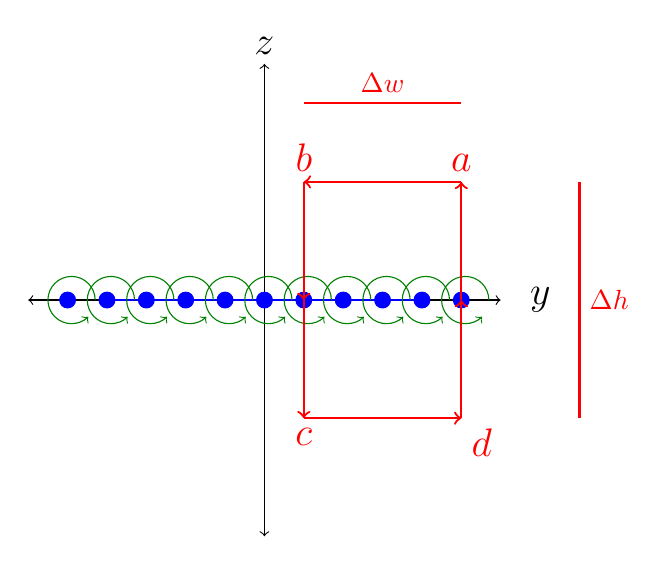
\begin{tikzpicture}
	
		%axis
		\draw[<->] (-3,0) --++ (6,0) node[right=0.25cm] {\Large$y$};
		\draw[<->] (0,-3) --++ (0,6) node[above] {\Large$z$};
		\draw[fill] (0,0) circle  (0.5mm) ;
%		\draw (0,0) circle (1mm) node[below left] {\Large$x$};
		
		% the sheet
		\draw[thick, blue] (-2,0) --++(4,0);
		
		% the currents coming out of the page
		\foreach \x in {-2.5,-2,...,2.5}{
			\draw[blue, fill=blue] (\x,0) circle (1mm);
			\draw[green!50!black, ->] (\x+0.35,0) arc (0:315:0.3);
		}
		
		% the magnetic field
%		\foreach \x in {-1.5,0,1.5}{
%			\draw[green!50!black, ->] (\x,0) arc (0:315:0.6);
%		}
		
		% contour segments
		\draw[red, ->, thick] (2.5,0) --++ (0,1.5) node[above] {\Large$a$};
		\draw[red, ->, thick] (2.5,1.5) --++ (-2,0) node[above] {\Large$b$};
		\draw[red, ->, thick] (0.5,1.5) --++ (0,-1.5);
		\draw[red, ->, thick] (0.5,0) --++ (0,-1.5) node[below] {\Large$c$};
		\draw[red, ->, thick] (0.5,-1.5) --++ (2,0) node[below right] {\Large$d$};
		\draw[red, ->, thick] (2.5,-1.5) --++ (0,1.5);
		\draw[red, thick] (0.5, 2.5) --++ (2,0) node[midway, above] {$\Delta w$};
		\draw[red, thick] (4,-1.5) --++ (0,3) node[midway, right] {$\Delta h$};

	\end{tikzpicture}
} % end scalebox
\end{textblock}
\begin{textblock}{7.5}(7,3)
	\begin{small}
	\eq{
		&\circled{1} \visible<0|handout:1>{\text{ Draw picture(s)} }\\[12pt]
		&\circled{2} \visible<0|handout:1>{\text{ Ampere's Law:}\; \oint_C \vec{H}\mycdot\vec{d\ell} = I_{\text{encls}} }\\[12pt]
		&\circled{3} \visible<0|handout:1>{ \;\vec{H} = \xhat H_{x} + \yhat H_{y} + \zhat H_z }\\[12pt]
		&\circled{4} \visible<0|handout:1>{\oint_C \vec{H}\mycdot \vec{d\ell} = \int_a^b \vec{H}\mycdot \vec{d\ell_1}  + \int_b^c \vec{H}\mycdot \vec{d\ell_2}} \\[12pt]
		& \visible<0|handout:1>{\qquad\qquad\qquad \int_c^d \vec{H}\mycdot \vec{d\ell_3}  + \int_d^a \vec{H}\mycdot \vec{d\ell_4} } \\
		&\visible<0|handout:1>{\qquad\qquad = \int_{\alert{\Delta w}}^{\alert{0}} \lp -\yhat H_y \rp \mycdot \lp \yhat dy \rp  + 0}\\
		&\visible<0|handout:1>{\qquad\qquad + \int_0^{\Delta w} \lp \yhat H_y \rp \mycdot \lp \yhat dy \rp  + 0 }\\[12pt]
		&\visible<0|handout:1>{\qquad\qquad = \handoutgap{0pt}{2H_y \Delta w} } 
	}
	\end{small}
\end{textblock}
\end{frame}

%%%%%%%%%%%%%%%%%%%%%%%%%%%%%%%%%%%%%%%%%%%%%%%%%%%%%%
%%%%%%%%%%%%%%%%%%%%%%%%%%%%%%%%%%%%%%%%%%%%%%%%%%%%%%

\begin{frame}{Ampere's Law: Sheet Charge}
\begin{textblock}{14.5}(0.5,3)
\scalebox{0.75}{
\tdplotsetmaincoords{70}{110}
\begin{tikzpicture}[tdplot_main_coords]
	% sheet charge
	\path[very thick, draw=blue, fill=blue!50!white, opacity=0.5] (2,0,-2) -- (-2,0,-2) -- (-2,0,2) -- (2,0,2) -- (2,0,-2); % sheet charge
	 \node[blue] at (-2,0.5,2) {$\rho_S$};
		
	%axes
	\coordinate (O) at (0,0,0);
	\draw[thick, <->] (-3.5,0,0) -- (3.5,0,0) node[anchor=north east]{$y$};
	\draw[thick,->] (0,0,0) --(0,3,0) node[right] {$z$}; 
	\draw[thick,<->] (0,0,-3) --(0,0,3) node[anchor=east]{$x$}; 
	
	\foreach \y in {-2,-1.5,...,2}{
		\draw[->,thick, thick, blue] (\y,0,-2) -- (\y,0,2);
	}
\end{tikzpicture}
} % end scalebox

\scalebox{0.5}{
	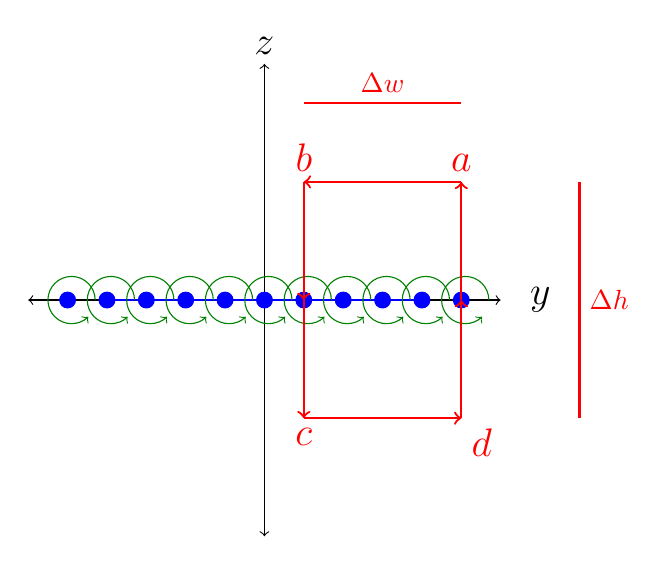
\begin{tikzpicture}
	
		%axis
		\draw[<->] (-3,0) --++ (6,0) node[right=0.25cm] {\Large$y$};
		\draw[<->] (0,-3) --++ (0,6) node[above] {\Large$z$};
		\draw[fill] (0,0) circle  (0.5mm) ;
%		\draw (0,0) circle (1mm) node[below left] {\Large$x$};
		
		% the sheet
		\draw[thick, blue] (-2,0) --++(4,0);
		
		% the currents coming out of the page
		\foreach \x in {-2.5,-2,...,2.5}{
			\draw[blue, fill=blue] (\x,0) circle (1mm);
			\draw[green!50!black, ->] (\x+0.35,0) arc (0:315:0.3);
		}
		
		% the magnetic field
%		\foreach \x in {-1.5,0,1.5}{
%			\draw[green!50!black, ->] (\x,0) arc (0:315:0.6);
%		}
		
		% contour segments
		\draw[red, ->, thick] (2.5,0) --++ (0,1.5) node[above] {\Large$a$};
		\draw[red, ->, thick] (2.5,1.5) --++ (-2,0) node[above] {\Large$b$};
		\draw[red, ->, thick] (0.5,1.5) --++ (0,-1.5);
		\draw[red, ->, thick] (0.5,0) --++ (0,-1.5) node[below] {\Large$c$};
		\draw[red, ->, thick] (0.5,-1.5) --++ (2,0) node[below right] {\Large$d$};
		\draw[red, ->, thick] (2.5,-1.5) --++ (0,1.5);
		\draw[red, thick] (0.5, 2.5) --++ (2,0) node[midway, above] {$\Delta w$};
		\draw[red, thick] (4,-1.5) --++ (0,3) node[midway, right] {$\Delta h$};

	\end{tikzpicture}
} % end scalebox
\end{textblock}
\begin{textblock}{7.5}(6,3)
	\eq{
		&\circled{6} \visible<0|handout:1>{\; I_{\text{encls}} = \oiint_S \vec{J}\mycdot \vec{dS} }\\[12pt]
		&\visible<0|handout:1>{\qquad = \int_0^{\Delta w} \xhat J_x \mycdot \xhat dy }\\[12pt]
		&\visible<0|handout:1>{\qquad = \handoutgap{0pt}{J_x \Delta w }}\\[12pt]
		&\visible<0|handout:1>{ H_{y} = \handoutgap{0pt}{ \dfrac{J_x}{2} } } 
	}
\end{textblock}
\end{frame}

%%%%%%%%%%%%%%%%%%%%%%%%%%%%%%%%%%%%%%%%%%%%%%%%%%%%%%
%%%%%%%%%%%%%%%%%%%%%%%%%%%%%%%%%%%%%%%%%%%%%%%%%%%%%%
\section{Solenoid}
\begin{frame}{Ampere's Law: Solenoid}
\begin{textblock}{7.5}(0,4)
	
	\includegraphics[scale=0.4]{ECE343/Bfield-single-coil}

\end{textblock}
\begin{textblock}{7.5}(8,5)

	\includegraphics[scale=0.25]{ECE343/solenoid-circuit}
	
\end{textblock}
\end{frame}

%%%%%%%%%%%%%%%%%%%%%%%%%%%%%%%%%%%%%%%%%%%%%%%%%%%%%%
%%%%%%%%%%%%%%%%%%%%%%%%%%%%%%%%%%%%%%%%%%%%%%%%%%%%%%
\begin{frame}{Ampere's Law: Solenoid}
\begin{textblock}{7.5}(0.5,2.5)
	
	\includegraphics[scale=0.35]{ECE343/Bfield-solenoid}
	
	\vspace{12pt}
	
	\includegraphics[scale=0.15]{ECE343/solenoid_cross-section}

\end{textblock}
\begin{textblock}{7.5}(7,3)

\begin{small}
	\eq{
		&\circled{1} \visible<0|handout:1>{\text{ Draw picture(s)} }\\[12pt]
		&\circled{2} \visible<0|handout:1>{ \text{ Ampere's Law:}\; \oint_C \vec{H}\mycdot\vec{d\ell} = I_{\text{encls}}}\\[12pt]
		&\circled{3} \visible<0|handout:1>{\;\vec{H} = \rhohat H_{\rho} + \phihat H_{\phi} + \zhat H_z }\\[12pt]
		&\circled{4} \visible<0|handout:1>{\oint_C \vec{H}\mycdot \vec{d\ell} = \int_A \vec{H}\mycdot \vec{d\ell_1}  + \int_B \vec{H}\mycdot \vec{d\ell_2}} \\[12pt]
		& \visible<0|handout:1>{\qquad\qquad\qquad \int_C \vec{H}\mycdot \vec{d\ell_3}  + \int_D \vec{H}\mycdot \vec{d\ell_4} } \\[12pt]
		&\visible<0|handout:1>{\qquad\qquad = \int_A \lp \zhat H_{z} \rp\mycdot\lp \zhat dz\rp + 0 + 0 + 0  } \\
		&\qquad\qquad = \visible<0|handout:1>{H_z \ell^{\prime} } \\[12pt]
		&\circled{5} \visible<0|handout:1>{ \; I_{\text{encls}}  =  \dfrac{N}{\ell} \ell^{\prime} I }\\[12pt]
		& \visible<0|handout:1>{ \vec{H} = \zhat H_z = \dfrac{N I }{\ell} }
	}
	\end{small}
\end{textblock}
\end{frame}

%%%%%%%%%%%%%%%%%%%%%%%%%%%%%%%%%%%%%%%%%%%%%%%%%%%%%%
%%%%%%%%%%%%%%%%%%%%%%%%%%%%%%%%%%%%%%%%%%%%%%%%%%%%%%
\section{Toroid}
\begin{frame}{Ampere's Law: Toroid}
\begin{textblock}{7}(0.5,3)
	
	\includegraphics[scale=0.25]{ECE343/toroid}

	\begin{scriptsize} 
	Note: the contour of integration is \textbf{inside} the core, meaning current through the surface defined by the contour is carried in the windings at the inner edge of the core:
	\end{scriptsize}
	
	\begin{center}
	\newsavebox{\myarrow}
	\savebox{\myarrow}{
		\begin{tikzpicture}
			\draw[red, ->] (0,0) --++(0,0.5);
		\end{tikzpicture}
	}
	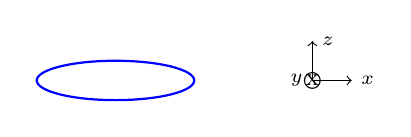
\begin{tikzpicture}
		
		%\draw[black, ultra thick] (0,0) --++ (2,0); 
%		\draw[black, thick] (0,0) ellipse (1cm and 0.25cm);
		\draw [thick, blue] (1,0) arc[start angle=0, end angle=360, x radius = 1cm, y radius = 0.25cm]
			\foreach  \x in {0, 0.07, ...,1}{
				node[pos=\x] {\usebox{\myarrow}}
			};
			
		\draw[->] (2.5,0) -- ++(0.5,0) node[right] {\scriptsize{$x$}};
		\draw[->] (2.5,0) --++ (0,0.5) node[right] {\scriptsize{$z$}};
		\draw (2.5,0) circle (1mm) node[left] {\scriptsize{$y$}};
		\node at (2.5,0) {\small{x}};
		
%		\foreach \x in {0,0.5,...,2}{
%			\draw[red, ->] (\x,-0.5) --++ (0,0.5); 
%		}
	
	\end{tikzpicture}
	\end{center}
	
\end{textblock}
\begin{textblock}{7.5}(7.5,2)

\begin{small}
	\eq{
		&\circled{1} \visible<0|handout:1>{\text{ Draw picture(s)} }\\[12pt]
		&\circled{2}  \visible<0|handout:1>{\text{ Ampere's Law:}\; \oint_C \vec{H}\mycdot\vec{d\ell} = I_{\text{encls}}}\\[12pt]
		&\circled{3} \visible<0|handout:1>{\;\vec{H} = \rhohat H_{\rho} + \phihat H_{\phi} + \zhat H_z}\\[12pt]
		&\circled{4} \visible<0|handout:1>{\oint_C  \vec{H}\mycdot \vec{d\ell} = \int_0^{2\pi} \vec{H}\mycdot \vec{d\ell_{\phi}}  }\\
		&\visible<0|handout:1>{\qquad\qquad = \int_0^{2\pi} \lp \phihat H_{\phi}\rp \mycdot \lp \phihat \rho d\phi \rp }\\
		&\visible<0|handout:1>{\qquad\qquad = \handoutgap{0pt}{2\pi \rho H_{\phi}}} \\
		&\circled{5} \visible<0|handout:1>{\; I_{\text{encls}}  = NI }\\
		&\visible<0|handout:1>{ \vec{H} = \phihat H_{\phi} = \dfrac{N I }{2\pi\rho} } 
	}
	\end{small}
\end{textblock}
\end{frame}

%%%%%%%%%%%%%%%%%%%%%%%%%%%%%%%%%%%%%%%%%%%%%%%%%%%%%%
%%%%%%%%%%%%%%%%%%%%%%%%%%%%%%%%%%%%%%%%%%%%%%%%%%%%%%
\begin{frame}{Maxwell's Equations: Static Fields}
\begin{textblock}{14.5}(0.5,5)
\begin{center}
\renewcommand{\arraystretch}{1.5}
\begin{tabular}{| l | c | c | }
	\hline
	\textbf{Law} 				& \textbf{Integral Form} 				& \textbf{Point Form} \\\hline\hline
	Gauss's Law for Electricity 	
		& $\oint_S \vec{E}\mycdot \vec{dS} = \dfrac{Q_{\text{encls}}}{\varepsilon}$ 	
		& $\mydiv{\vec{E}} = \dfrac{\rho}{\varepsilon_v} $
	\\\hline
	Gauss's Law for Magnetism 	
		& $\oint_S \vec{B} \mycdot \vec{dS} = 0$
		& $\mydiv{\vec{B}}  = 0 $
	\\\hline
	Faraday's Law	
		& $\oint_S \vec{E}\mycdot \vec{d\ell} =  0$
		& $\curl{\vec{E}} = 0 $
	\\\hline
	Ampere's Law
		&$\oint_S \vec{H}\mycdot \vec{d\ell} = I_{\text{encl}} $
		&$\curl{\vec{H}} = \vec{J} $
	\\\hline
\end{tabular}	
\end{center}
\end{textblock}
\end{frame}
\begin{comment}
\end{comment}